\chapter{Induction and Invariants}

Induction is the workhorse that never gets top billing. In our tagged SIGMOD'26 corpus, 36 of 228 papers use it (the \#3 tool overall); the pairing \emph{correctness}~$\times$~\emph{induction}, with 29 papers, is the single most frequent property--tool co-occurrence in the survey, and induction also powers the \emph{upper-bound} pairing in 21 papers. The characteristic shape is not one grand named theorem but thousands of small, unnamed invariants --- half-page lemmas saying that one more elimination step, recursive call, or rewrite keeps a component consistent. Induction is thus the instrument of \emph{component} correctness: each cache, rewrite rule, or decomposition step is verified locally, and the global guarantee is assembled from the local ones.

\section{The Tool: Induction on What?}

Every inductive argument in the corpus answers two questions: what do we induct on, and what is preserved at each step?

\paragraph{Induction on what?} Three substrates dominate.

\begin{enumerate}
\item \textbf{Execution steps.} An algorithm induces a sequence of states $s_0, s_1, \dots, s_t$, one per operation (a function call, an elimination, a rewrite). One proves a state predicate $I$ --- the \emph{invariant} --- by induction on $i$: $I(s_0)$ holds, and each operation preserves $I$, so $I$ holds in every reachable state and implies the specification at final states. This is the inductive-assertion method of Floyd~\cite{induction-bg1} and Hoare~\cite{induction-bg2}, the loop-invariant discipline of algorithms texts~\cite{induction-bg4}, and Manna--Pnueli \emph{safety} reasoning: nothing bad ever becomes true~\cite{induction-bg3}.
\item \textbf{Structural recursion.} The object is built recursively --- a tree decomposition, an elimination forest, a recursive pseudo-tree, a hierarchy --- and the property is proved on the whole from the property on the parts. The database workhorse is \emph{leaf-peeling}: remove a leaf bag or leaf vertex, apply the induction hypothesis to the smaller object, then extend by one step.
\item \textbf{A natural-number measure.} Strong induction on a quantity that strictly decreases: the number of eliminated nodes, the number of bags, or the length of a rewrite sequence; structural induction is routinely converted into this form by choosing a measure~\cite{induction-bg5}.
\end{enumerate}

\begin{example}[Invariant preservation]
Given a set of states $\Sigma$, an initial state $s_0$, and a set of operations $\Gamma$, a predicate $I \subseteq \Sigma$ is an \emph{invariant} if (i) $I(s_0)$ holds, and (ii) whenever $I(s)$ holds and $s'$ results from applying an operation of $\Gamma$ to $s$, then $I(s')$ holds. By induction on the number of executed operations, every reachable state satisfies $I$; any property implied by $I$ at final states is therefore guaranteed.
\end{example}

\begin{center}
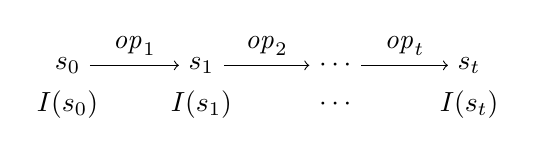
\begin{tikzpicture}
\node (s0) at (0,0)   {$s_0$};
\node (s1) at (1.7,0) {$s_1$};
\node (d)  at (3.4,0) {$\cdots$};
\node (st) at (5.1,0) {$s_t$};
\draw[->] (s0) -- node[above]{$\mathit{op}_1$} (s1);
\draw[->] (s1) -- node[above]{$\mathit{op}_2$} (d);
\draw[->] (d)  -- node[above]{$\mathit{op}_t$} (st);
\node at (0,-0.5)   {$I(s_0)$};
\node at (1.7,-0.5) {$I(s_1)$};
\node at (3.4,-0.5) {$\cdots$};
\node at (5.1,-0.5) {$I(s_t)$};
\end{tikzpicture}\\[2pt]
{\small Base case $I(s_0)$; every operation preserves $I$; hence $I$ holds at every step, and $I(s_t)$ implies the specification.}
\end{center}

\paragraph{Structural versus strong induction.} Structural induction follows the formation rules of a data structure ($P$ on the immediate substructures yields $P$ on the structure); strong induction on the naturals assumes $P(j)$ for all $j < k$ to derive $P(k)$. The two are interderivable via a measure such as the number of bags of a decomposition; one picks whichever form makes the step case a purely local check.

\section{Exemplars from the Corpus}

\paragraph{Induction on elimination steps.}
Exact resistance-distance computation on graphs of small treewidth eliminates the nodes of a tree decomposition one at a time, updating a pseudo-inverse matrix that must retain a precise block shape \cite{sigmod26-307}.

\begin{lemma}[Elimination state]
Let $G$ be a graph with Laplacian $L$, and let $U_1 \subseteq U_2 \subseteq V$ be sets of nodes. After the elimination of the nodes of $U_2 \setminus U_1$, the state matrix satisfies
\[
S_{|U_2 \setminus U_1|} \;=\;
\begin{pmatrix} L^{-1}_{U_1 U_1} & 0 \\ 0 & 0 \end{pmatrix}.
\]
\end{lemma}

The induction variable is the number of eliminated nodes, and the induction hypothesis is stated as an explicit invariant of the state: after eliminating $k$ nodes (base case $S_0 = L^{-1}_{U_2 U_2}$), all rows and columns of eliminated nodes are zero, and the block on the surviving nodes is exactly the Schur complement of the remaining nodes \cite{sigmod26-307}.

\paragraph{Induction on the run, and on bags.}
Charting which space--time exponent pairs are feasible for sum--product queries requires algorithms that evaluate a query along a recursive pseudo-tree (RPT) with per-vertex caches \cite{sigmod26-371}.

\begin{lemma}[Cache invariant]
Let $\mathcal{T}$ be a recursive pseudo-tree (RPT) of the sum--product query $Q$, and let $A$ be an arbitrary vertex of $\mathcal{T}$. Then, during the execution of the algorithm, the function call $\mathrm{solve}(A, \mathbf{x})$ returns the answer to the subquery of $Q$ at $A$, restricted to the part of the partial assignment $\mathbf{x}$ that is over the variables of $A$; furthermore, after the subsequent $\mathrm{fillCache}$ call, the cache $M_A$ holds exactly this value.
\end{lemma}

The induction is over the sequence of function calls of a run: the invariant is that every completed $\mathrm{solve}$/$\mathrm{fillCache}$ pair leaves $M_A$ storing precisely the restricted subquery answer. The companion plan-dominance proof is structural, proceeding by induction on the number of bags of a tree decomposition: peel a leaf bag, eliminate the variables in that bag but not in its parent's, and apply the hypothesis to the smaller decomposition \cite{sigmod26-371}.

\paragraph{Induction on rewrite sequences.}
A unifying algorithm for hierarchical queries computes full symbolic provenance once and transports it to any target algebra by a homomorphism; its correctness rests on a two-rule elimination procedure on the query itself \cite{sigmod26-264}.

\begin{proposition}[Elimination procedure for hierarchical queries]
A query $Q$ is hierarchical if and only if the following elimination procedure transforms $Q$ into a query with a single nullary atom, i.e.\ of the form \texttt{Q() :- R()}. Repeatedly apply one of the following two rules, until neither rule applies:
\begin{itemize}
\item[\textup{(Rule 1)}] Eliminate a ``private'' variable: find a variable $Y \in \mathrm{vars}(Q)$ that occurs in only one atom $R(\mathbf{X})$ in $Q$, and replace $R(\mathbf{X})$ with $R'(\mathbf{X} \setminus \{Y\})$, where $R'$ is a new relation symbol.
\item[\textup{(Rule 2)}] Eliminate a ``duplicate atom'': find two distinct atoms $R_1(\mathbf{X})$, $R_2(\mathbf{X})$ over the same variables $\mathbf{X}$ and replace the two by a single atom.
\end{itemize}
\end{proposition}

The induction variable is the length of the rewrite sequence, and the invariant holds in both directions: a hierarchical query not yet of the form \texttt{Q() :- R()} always admits Rule 1 or Rule 2 and stays hierarchical, while either rule applied to a non-hierarchical query leaves it non-hierarchical. The same stepwise induction carries the provenance theorem --- after each rule application, the output is the $\varphi$-image of the symbolically annotated one \cite{sigmod26-264}.

\paragraph{Bottom-up induction over the query tree.}
Do regular-path atoms make acyclic conjunctive queries harder to evaluate than relational ones? For combinatorial algorithms the answer is no, and the guarantee is quantitative \cite{sigmod26-011}\pods.

\begin{theorem}[Acyclic CRPQ evaluation]
Let $Q$ be any acyclic CRPQ, and $G$ be an input edge-labeled graph of size $N$. Then $Q$ over $G$ can be answered in time
\[
O\bigl(N + N \cdot \mathrm{OUT}^{\,1 - 1/\max(\textsf{fn-fhtw}(Q),\,2)} + \mathrm{OUT}\bigr)
\]
in data complexity, where $\mathrm{OUT}$ is the output size and \textsf{fn-fhtw}$(Q)$ is the free-connex fractional hypertree width of $Q$.
\end{theorem}

Correctness and runtime are proved together by bottom-up induction over the acyclic structure of $Q$ (reduced first to bound-connected components and free-leaf CRPQs): the invariant at each subtree is that the partial evaluation materializes exactly the answers of the subquery rooted there, with heavy/light splitting keeping every intermediate within the budget $\Delta = \mathrm{OUT}^{1-1/\ell}$ \cite{sigmod26-011}\pods.

\begin{reachbox}{When to reach for induction}
\begin{itemize}
\item A component has state evolving by local steps and the claim is ``nothing drifts'' --- caches, elimination pipelines, rewrite rules. The property is a safety property: prove an invariant over the state, not a formula about the final value.
\item Choose the induction variable first: execution steps for imperative components; the recursive structure (tree decomposition, pseudo-tree, hierarchy) for recursive ones. Leaf-peeling is the default move on trees.
\item Make the invariant strong enough to imply the specification. If the step case will not close, strengthen it (add the block shape, the cache contents, hierarchality) --- strengthening is the normal iteration of the method, not a failure.
\item Pair the invariant with a strictly decreasing measure (bags, nodes, or rule applications left) to obtain termination and runtime bounds --- this is how induction also powers the \emph{upper-bound} pairing (21 papers).
\item Audit the step case over \emph{every} operation, and check the trivial base cases (empty input, single bag, zero eliminations): one missed case silently breaks the entire argument.
\end{itemize}
\end{reachbox}
